% !Mode:: "TeX:UTF-8"%确保文档utf-8编码
%commands:
%environments:  
\documentclass[xetex,compress]{mybeamer}
%8pt, 9pt, 10pt, 11pt, 12pt, 14pt, 17pt, 20pt
%draft – no graphics, footlines,...
%handout – no overlays
%xcolor=x11names – define more names for colors
%,aspectratio=169
%compress the navagationbar  change to one line

\usetheme{Singapore}
\usecolortheme{rose}
%albatross fly crane seagull beetle wolverine dove beaver
% innercolortheme lily orchid rose               the colors of blocks. 
%outer color theme whale seahorse dolphin          headline, footline, and sidebar
\usefonttheme{serif}

\title{制作幻灯片示例}
\subtitle{基于xelatex指南}
%\date
%\institute
%\logo
\author{万泽}
\date{2013年12月20日}

\begin{document}

\begin{frame}
\titlepage
\end{frame}
%plain  for large firgure  , fragile   can catcode ,mainly for verbatim environment


\begin{frame}
\frametitle{目录}
\setcounter{tocdepth}{1}
\tableofcontents[pausesections]%pausesections section pause
\end{frame}

%<1>  first show <2> second show [<+->]依次显示 <1-2>1,2都显示 <1->从1一直显示


\section{前言}%beamer class divided into section subsection subsubsection
%section* etc add to navigation bars not the toc
\subsection{引言}
\begin{frame}
\frametitle{引言}
\begin{block}{}
要将幻灯片写成一个系统的指南或者手册而利用幻灯片的形式多少有点不伦不类,反正源码在github上是可以见到的,所以我干脆将各种可见元素组合或者样式表现出来,需要的就看源码就是了。本幻灯片自建了一个mybeamer.cls,放置目录为:texmf/tex/latex/base/mybeamer.cls。其中大部分xelatex指南中而来的配置都删除了,因为不适合这里。除了字体的配置继续有效之外。
\end{block}
\end{frame}


\subsection{光催化机理}
\begin{frame}
\frametitle{光催化机理}
\begin{columns}
\column{0.5\textwidth}
\begin{block}{}
\centering
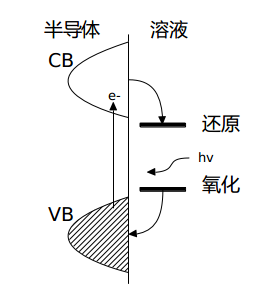
\includegraphics[scale=0.6]{figures/光催化机理图} 
\end{block}
\column{0.5\textwidth}
\begin{block}{}
半导体有一个禁带能宽,当照射进来的光的能量超过禁带能宽时,就会把价带(VB)的电子激发并进入导带(CB)。这样在价带会形成空穴,而在导带会形成额外的电子,通常这些空穴—电子对是成对出现的。
\end{block}
\end{columns}
\end{frame}


\begin{frame}
\frametitle{Fujishima的开创性工作}
\begin{block}{}
\centering
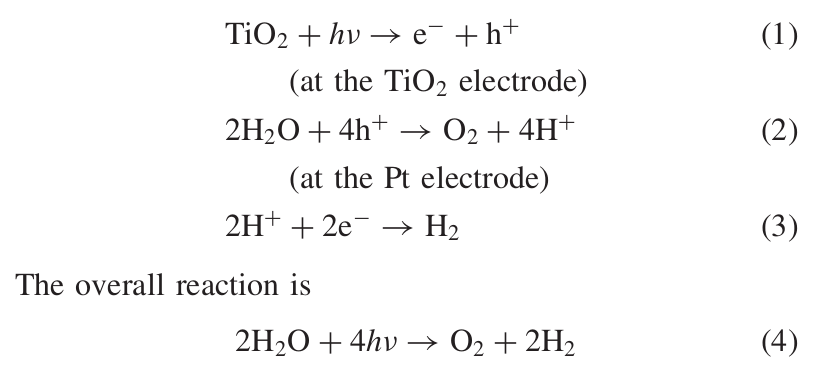
\includegraphics[scale=0.3]{figures/光分解水化学反应式} 
\end{block}
\begin{block}{}
其中\chemfig{\mathbf{TiO_2}}是光电阳极释放电子,Pt是光电阴极在这里释放氧气。整个反应就是水的分解反应。这个光化学电池量子效率是非常低下的,大约为0.1。
\end{block}
\end{frame}

















\end{document}
